\section{Localização}
\label{sec:luz-estruturada}

	As informações provenientes do rastreamento de uma entidade servem como base para que a localização da mesma possa ser obtida. Com essas informações é possível determinar os pontos da imagem que representam a entidade e calcular as distâncias dos mesmos em relação a câmera utilizada na captura das imagens. Este cálculo consiste em uma tarefa relevante em sistemas de computação visual~\cite{jain}. Para isso,
	deve-se obter informações de profundidade das entidades em interesse. Essas
	informações podem ser obtidas utilizando imagens de intensidade ou de
	profundidade.
	
	Uma maneira comum de se obter informações de profundidade de imagens de
	intensidade é adquirir um par de imagens usando duas câmeras deslocadas entre si
	por uma distância conhecida. Como alternativa, duas ou mais imagens obtidas de
	uma câmera em movimento também podem ser utilizadas para calcular informações de
	profundidade~\cite{jain}. Esse método é conhecido como \textit{Stereo Vision} e
	necessita ser bem calibrado.  Além disso, os algoritmos que implementam este método
	geralmente são computacionalmente custosos e não funcionam em ambiente com baixa
	condição de iluminação~\cite{fall-detection}.
	
	Informações de profundidade também podem ser obtidas indiretamente através de
	imagens de intensidade utilizando sinais na imagem, como sombreamento e
	textura~\cite{jain}.
	
	Ao contrário das imagens de intensidade, imagens cujo valor em cada pixel é uma
	função da distância do ponto correspondente na cena do sensor são chamadas de
	imagens de profundidade, exemplificada na Figura \ref{depthimage}. Estas imagens
	podem ser adquiridas diretamente utilizando sensores específicos~\cite{jain}.
	Alguns dos métodos para se obter imagens de profundidade mais conhecidos são:

	\begin{figure}[htb]
		\begin{center}
			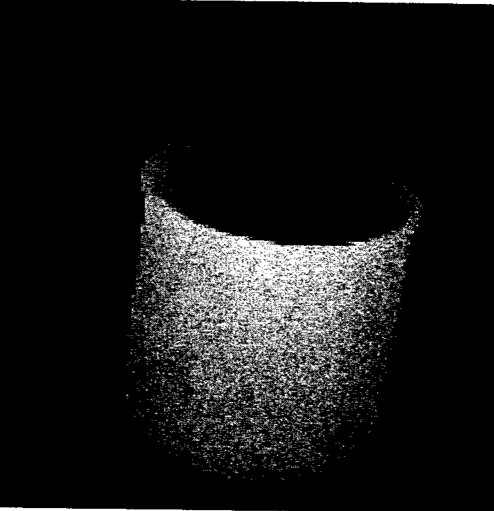
\includegraphics[scale=0.3]{figuras/2.FundamentacaoTeorica/depthimage.png}
		\end{center}
		\caption{Imagem de profundidade de uma caneca de café~\cite{jain}.}
		\label{depthimage}
	\end{figure}

	\begin{enumerate}
		\item \textbf{Triangulação:} utiliza as propriedades geométricas do triângulo
		para calcular a localização de entidades. Pode ser dividida em duas
		subcategorias~\cite{triangulacao}: 
			\begin{itemize}
				\item \textbf{lateração}: computa a posição de uma
		entidade estimando sua distância de múltiplos ponto de referência. Calcular a
		posição de uma entidade em duas dimensões requer estimativas de distância de
		três pontos não colineares como mostrado na Figura \ref{fig:lateration}. Nesta figura, para se obter a localização da entidade X é necessário obter a distância entre a mesma e três pontos de referência não colinerares.
				\item \textbf{angulação}: utiliza
		ângulos para determinar a localização da entidade. Em geral, angulação em duas
		dimensões requer estimativas de dois ângulos e a estimativa da distância entre
		dois pontos de referência como mostrado na Figura
		\ref{fig:angulation}. Nesta figura, para se se localizar a
			entidade $\displaystyle X$ utiliza-se ângulos relativos a um vetor de
			referência $\displaystyle 0º$ e a distância entre dois pontos de referência;
			\end{itemize}

		
		\begin{figure}[htb]
			\begin{center}
				\subfloat[Lateração] {
					\label{fig:lateration}
					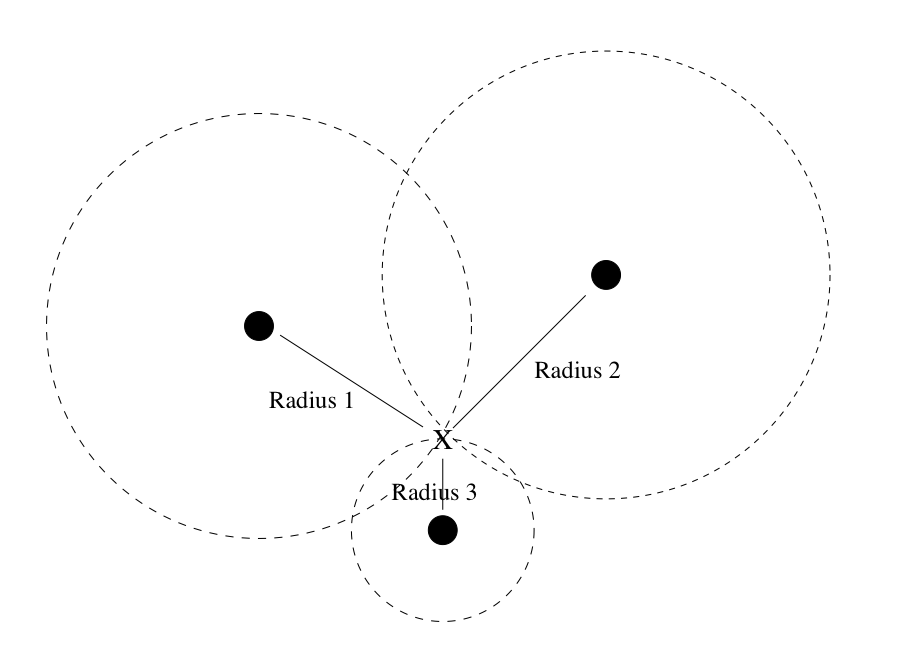
\includegraphics[width=0.45\textwidth]{figuras/2.FundamentacaoTeorica/lateration.png}}
				\subfloat[Angulação] {
					\label{fig:angulation}
					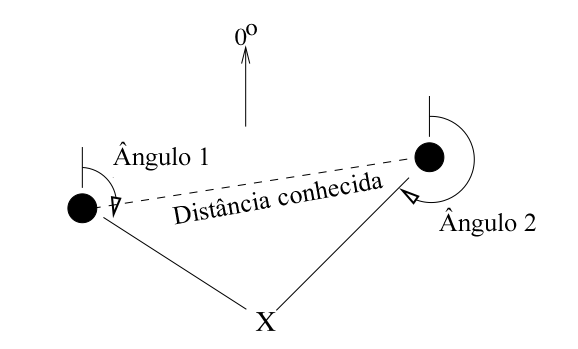
\includegraphics[width=0.45\textwidth]{figuras/2.FundamentacaoTeorica/angulation.png}}
			\end{center}
			\caption{ (a) Exemplo de Lateração~\cite{triangulacao}. (b)Exemplo de Angulação~\cite{triangulacao}.}
		\end{figure}

		\item \textbf{Tempo de Vôo (TOF - \textit{Time of flight}):} a distância até a
		entidade é calculada observando a diferença de tempo entre o pulso
		eletromagnético transmitido e recebido. A informação de profundidade também pode
		ser obtida através da detecção da diferença de fase entre as ondas transmitidas
		e as recebidas de um feixe de amplitude modulada~\cite{jain, fall-detection}.
		Câmeras TOF provêem imagens de profundidade com melhor acurácia em relação ao
		método de \textit{Stero Vision}, porém são muito caras e pouco
		acessíveis~\cite{fall-detection};
		
		\item \textbf{Luz Estruturada:} uma imagem de
		profundidade não pode ser obtida utilizando somente um sensor de vídeo. Porém,
		adicionando uma textura artificial na cena, como na
		Figura~\ref{fig:structured-light}, uma imagem de profundidade pode ser
		recuperada. Esse princípio consiste na projeção de pontos de luz infra-vermelhos
		na cena que são recuperados por uma câmera infra-vermelha que lê a textura.
		Trata-se de um método mais acessível que o TOF, porém é pouco eficiente
		para estimar a distância dos pontos nas bordas dos objetos e em posições muito
		longe do sensor~\cite{fall-detection};
		
		\begin{figure}[H]
			\begin{center}
				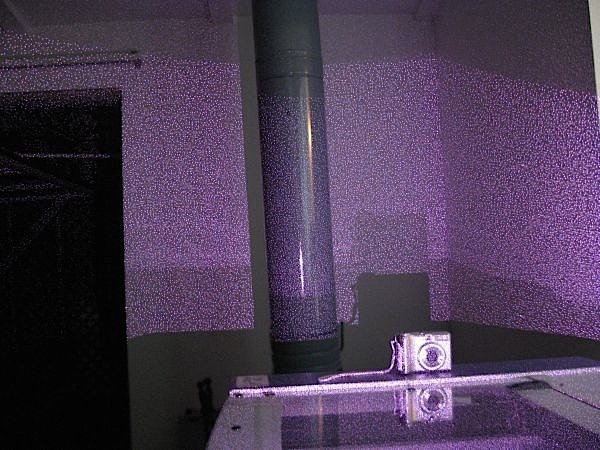
\includegraphics[width=0.45\textwidth]{figuras/2.FundamentacaoTeorica/structured-light.jpg}
			\end{center}
			\caption{Exemplo de uma textura artificial adicionada a cena por meio de
			pontos de luz infra-vermelha utilizando o método Luz Estruturada~\cite{img-strutuctured-light}.}
			\label{fig:structured-light}
		\end{figure}
	\end{enumerate}

	Imagens de profundidade são úteis devido a sua especificação explícita de
	valores de profundidade. Ao mesmo tempo acreditava-se que se a informação de
	profundidade fosse disponibilizada de maneira explícita, o processamento
	posterior da imagem seria facilitado. Tornou-se claro que a informação de
	profundidade ajuda, porém a tarefa básica de interpretação de imagens mantém
	todas as suas dificuldades~\cite{jain}.

